\section{不同中心度不同质量区间中温度抽取结果}

相比于STAR 束流能量扫描第一阶段(Beam Energy Scan Phase I, BES-I)的测量,\sNN = 54.4 GeV和 27 GeV的测量一个很大的优势就是有着更多的统计量,可以进行在不同中心度下的双电子谱的测量,基于此,在本分析当中对低质量区间和中等质量区间不同中心度下的双电子谱都进行了和前文当中相同的拟合来抽取介质的温度。

图\ref{fig:T_vs_Npart_Run17_54GeV}总结了在不同中心度下的温度抽取的结果。可以看到,在不同的中心度下相同的质量区间内的拟合结果所抽取的温度并没有明显的中心度的依赖。同时相同的质量区间内抽取的温度在不同的中心度区间也互相符合的很好。在低质量区间当中抽取的温度均在为170 MeV附近,接近理论计算中得到的夸克胶子等离子体的相变温度${\rm T_{pc} = 156 \pm 1.5 ~MeV}$。而在中等质量区间,不同中心度抽取得到的温度在各个中心度下均高于在低质量区间抽取得到的温度以及格点量子色动力学中计算得到的夸克胶子等离子体的相变温度。

\begin{figure}[htb]
    \begin{center}
    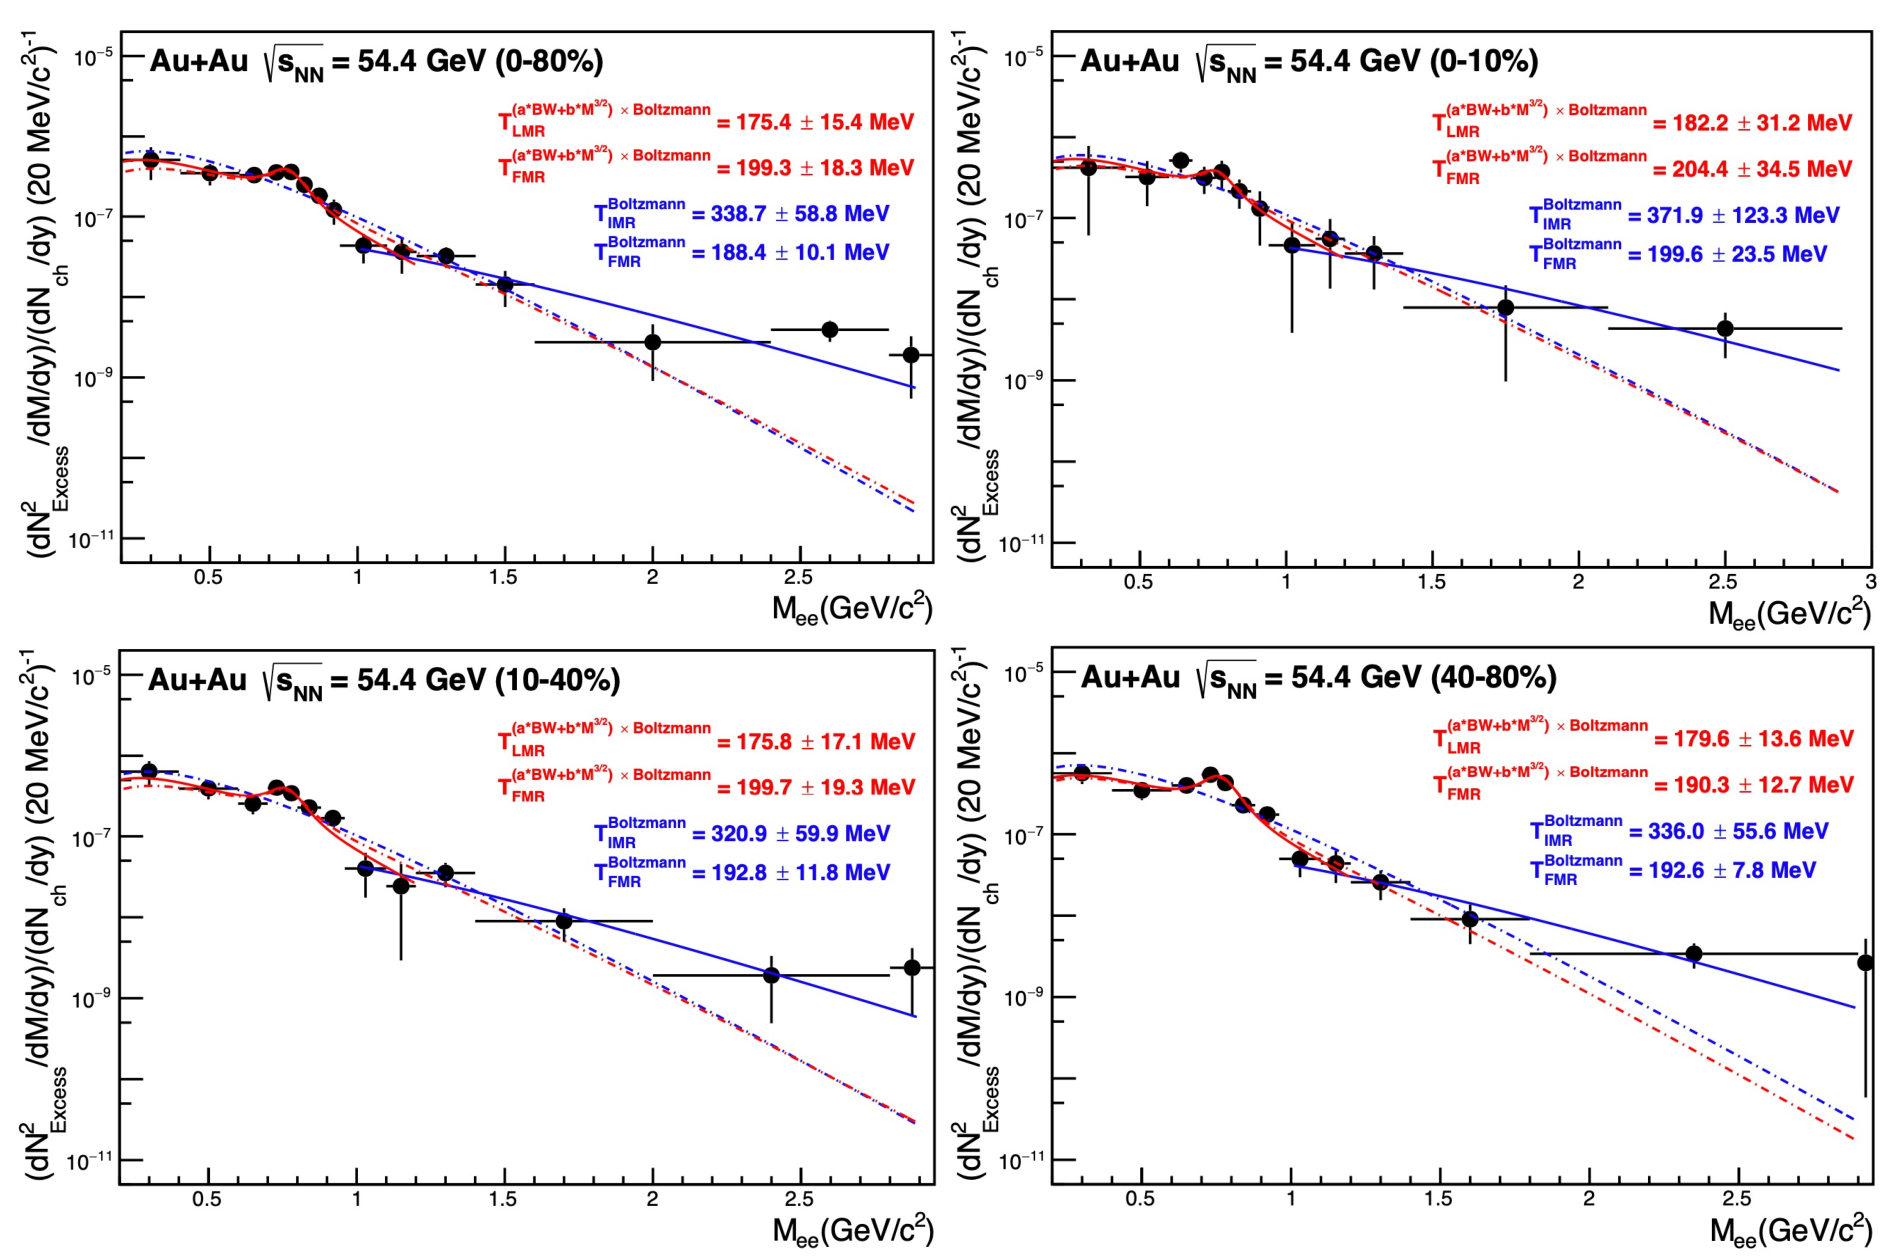
\includegraphics[width=0.75\textwidth,clip]{figures/Chapter4/Excess_fit.pdf}
    \end{center}
    \caption[\sNN = 54.4 GeV金-金对撞当中不同中心度下双电子额外产额谱及拟合结果示意图]{\sNN = 54.4 GeV金-金对撞当中不同中心度下双电子额外产额谱及拟合结果示意图,采用的拟合区间和拟合方程在图中进行标示。}
    \label{fig:Excess_fit}
\end{figure}

\begin{figure}[htb]
    \begin{center}
    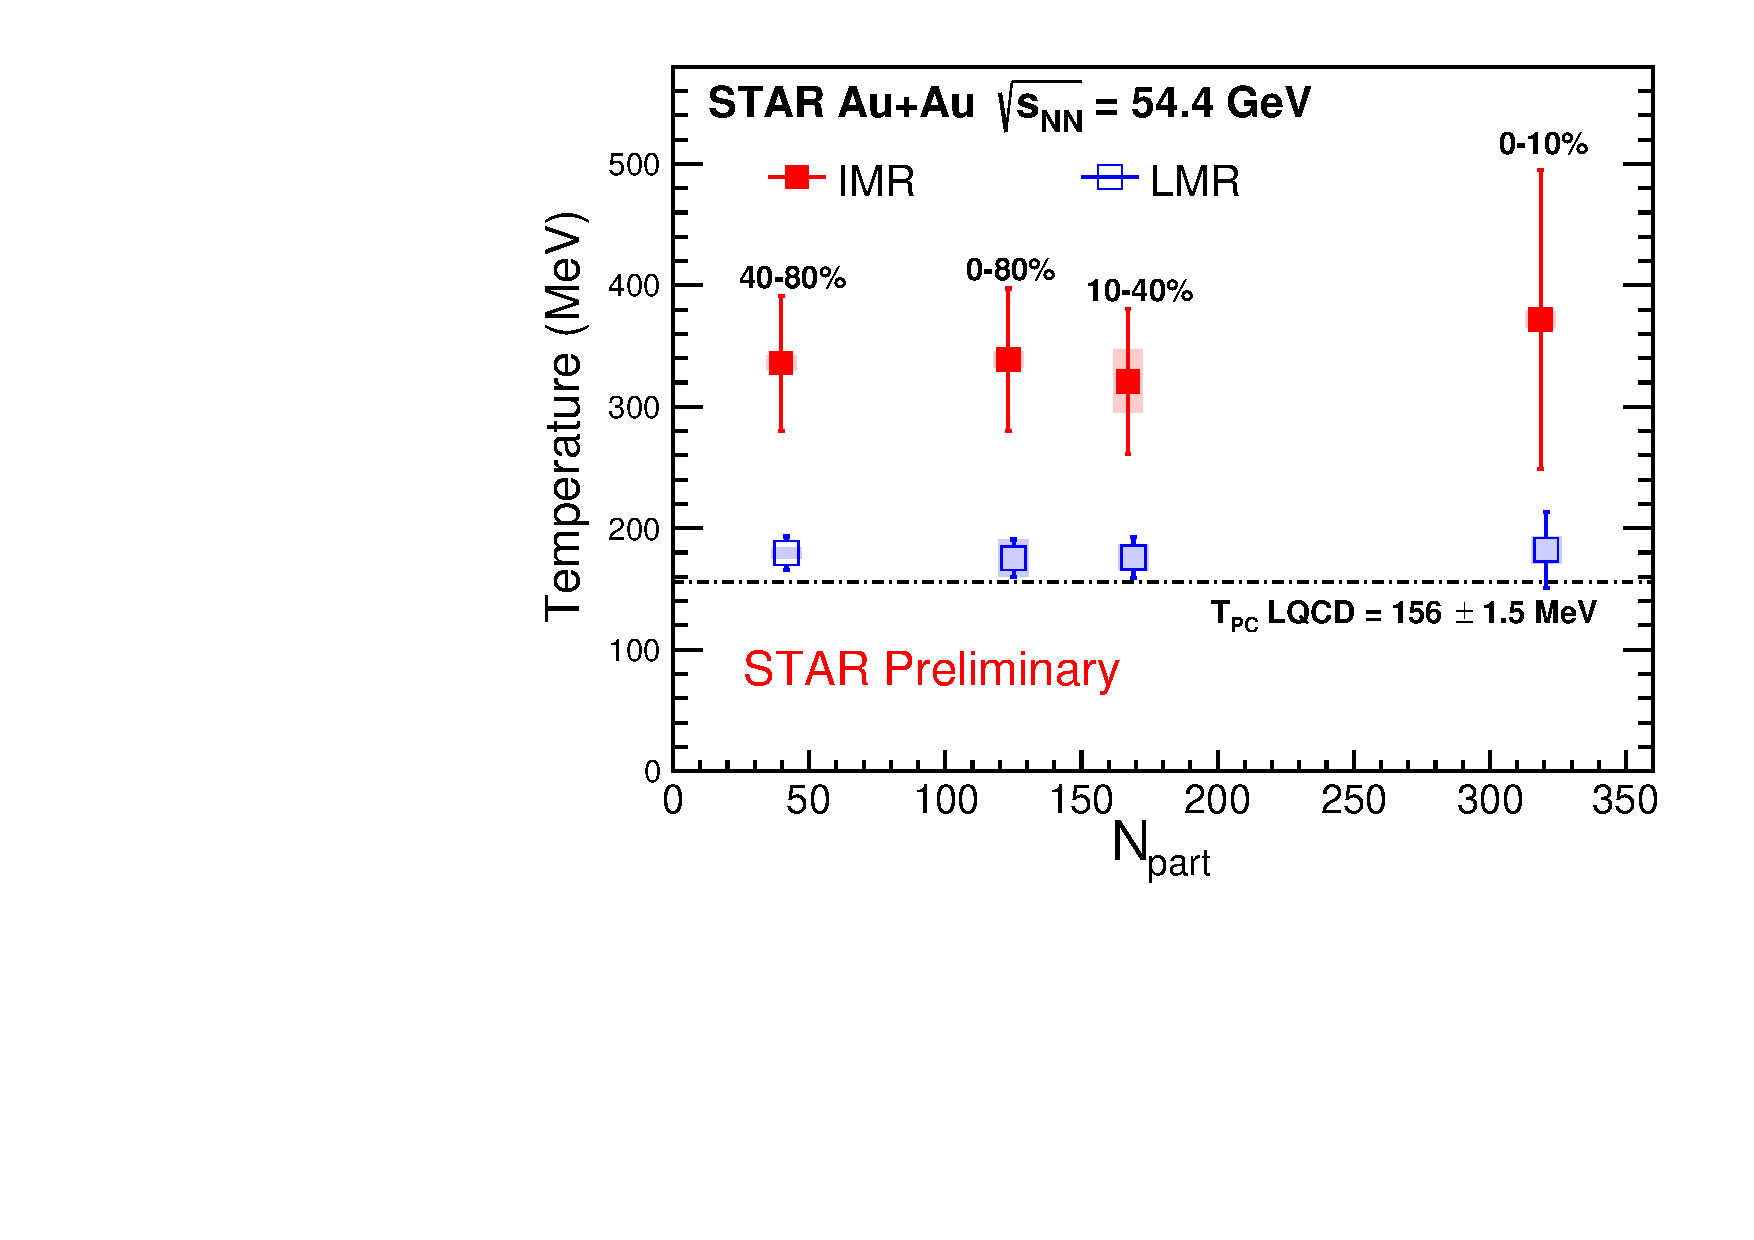
\includegraphics[width=0.75\textwidth,clip]{figures/Chapter4/T_vs_Npart_Run17_54GeV.pdf}
    \end{center}
    \caption[STAR实验中 \sNN = 54.4 GeV金-金对撞不同中心度下温度抽取比较示意图]{STAR实验中 \sNN = 54.4 GeV金-金对撞不同中心度下温度抽取比较示意图}
    \label{fig:T_vs_Npart_Run17_54GeV}
\end{figure}